% Options for packages loaded elsewhere
\PassOptionsToPackage{unicode}{hyperref}
\PassOptionsToPackage{hyphens}{url}
\PassOptionsToPackage{dvipsnames,svgnames,x11names}{xcolor}
%
\documentclass[
  letterpaper,
  DIV=11,
  numbers=noendperiod]{scrartcl}

\usepackage{amsmath,amssymb}
\usepackage{setspace}
\usepackage{iftex}
\ifPDFTeX
  \usepackage[T1]{fontenc}
  \usepackage[utf8]{inputenc}
  \usepackage{textcomp} % provide euro and other symbols
\else % if luatex or xetex
  \usepackage{unicode-math}
  \defaultfontfeatures{Scale=MatchLowercase}
  \defaultfontfeatures[\rmfamily]{Ligatures=TeX,Scale=1}
\fi
\usepackage{lmodern}
\ifPDFTeX\else  
    % xetex/luatex font selection
\fi
% Use upquote if available, for straight quotes in verbatim environments
\IfFileExists{upquote.sty}{\usepackage{upquote}}{}
\IfFileExists{microtype.sty}{% use microtype if available
  \usepackage[]{microtype}
  \UseMicrotypeSet[protrusion]{basicmath} % disable protrusion for tt fonts
}{}
\makeatletter
\@ifundefined{KOMAClassName}{% if non-KOMA class
  \IfFileExists{parskip.sty}{%
    \usepackage{parskip}
  }{% else
    \setlength{\parindent}{0pt}
    \setlength{\parskip}{6pt plus 2pt minus 1pt}}
}{% if KOMA class
  \KOMAoptions{parskip=half}}
\makeatother
\usepackage{xcolor}
\setlength{\emergencystretch}{3em} % prevent overfull lines
\setcounter{secnumdepth}{-\maxdimen} % remove section numbering
% Make \paragraph and \subparagraph free-standing
\ifx\paragraph\undefined\else
  \let\oldparagraph\paragraph
  \renewcommand{\paragraph}[1]{\oldparagraph{#1}\mbox{}}
\fi
\ifx\subparagraph\undefined\else
  \let\oldsubparagraph\subparagraph
  \renewcommand{\subparagraph}[1]{\oldsubparagraph{#1}\mbox{}}
\fi


\providecommand{\tightlist}{%
  \setlength{\itemsep}{0pt}\setlength{\parskip}{0pt}}\usepackage{longtable,booktabs,array}
\usepackage{calc} % for calculating minipage widths
% Correct order of tables after \paragraph or \subparagraph
\usepackage{etoolbox}
\makeatletter
\patchcmd\longtable{\par}{\if@noskipsec\mbox{}\fi\par}{}{}
\makeatother
% Allow footnotes in longtable head/foot
\IfFileExists{footnotehyper.sty}{\usepackage{footnotehyper}}{\usepackage{footnote}}
\makesavenoteenv{longtable}
\usepackage{graphicx}
\makeatletter
\def\maxwidth{\ifdim\Gin@nat@width>\linewidth\linewidth\else\Gin@nat@width\fi}
\def\maxheight{\ifdim\Gin@nat@height>\textheight\textheight\else\Gin@nat@height\fi}
\makeatother
% Scale images if necessary, so that they will not overflow the page
% margins by default, and it is still possible to overwrite the defaults
% using explicit options in \includegraphics[width, height, ...]{}
\setkeys{Gin}{width=\maxwidth,height=\maxheight,keepaspectratio}
% Set default figure placement to htbp
\makeatletter
\def\fps@figure{htbp}
\makeatother
\newlength{\cslhangindent}
\setlength{\cslhangindent}{1.5em}
\newlength{\csllabelwidth}
\setlength{\csllabelwidth}{3em}
\newlength{\cslentryspacingunit} % times entry-spacing
\setlength{\cslentryspacingunit}{\parskip}
\newenvironment{CSLReferences}[2] % #1 hanging-ident, #2 entry spacing
 {% don't indent paragraphs
  \setlength{\parindent}{0pt}
  % turn on hanging indent if param 1 is 1
  \ifodd #1
  \let\oldpar\par
  \def\par{\hangindent=\cslhangindent\oldpar}
  \fi
  % set entry spacing
  \setlength{\parskip}{#2\cslentryspacingunit}
 }%
 {}
\usepackage{calc}
\newcommand{\CSLBlock}[1]{#1\hfill\break}
\newcommand{\CSLLeftMargin}[1]{\parbox[t]{\csllabelwidth}{#1}}
\newcommand{\CSLRightInline}[1]{\parbox[t]{\linewidth - \csllabelwidth}{#1}\break}
\newcommand{\CSLIndent}[1]{\hspace{\cslhangindent}#1}

\usepackage{booktabs}
\usepackage{caption}
\usepackage{longtable}
\usepackage{colortbl}
\usepackage{array}
\KOMAoption{captions}{tableheading}
\makeatletter
\makeatother
\makeatletter
\makeatother
\makeatletter
\@ifpackageloaded{caption}{}{\usepackage{caption}}
\AtBeginDocument{%
\ifdefined\contentsname
  \renewcommand*\contentsname{Table of contents}
\else
  \newcommand\contentsname{Table of contents}
\fi
\ifdefined\listfigurename
  \renewcommand*\listfigurename{List of Figures}
\else
  \newcommand\listfigurename{List of Figures}
\fi
\ifdefined\listtablename
  \renewcommand*\listtablename{List of Tables}
\else
  \newcommand\listtablename{List of Tables}
\fi
\ifdefined\figurename
  \renewcommand*\figurename{Figure}
\else
  \newcommand\figurename{Figure}
\fi
\ifdefined\tablename
  \renewcommand*\tablename{Table}
\else
  \newcommand\tablename{Table}
\fi
}
\@ifpackageloaded{float}{}{\usepackage{float}}
\floatstyle{ruled}
\@ifundefined{c@chapter}{\newfloat{codelisting}{h}{lop}}{\newfloat{codelisting}{h}{lop}[chapter]}
\floatname{codelisting}{Listing}
\newcommand*\listoflistings{\listof{codelisting}{List of Listings}}
\makeatother
\makeatletter
\@ifpackageloaded{caption}{}{\usepackage{caption}}
\@ifpackageloaded{subcaption}{}{\usepackage{subcaption}}
\makeatother
\makeatletter
\@ifpackageloaded{tcolorbox}{}{\usepackage[skins,breakable]{tcolorbox}}
\makeatother
\makeatletter
\@ifundefined{shadecolor}{\definecolor{shadecolor}{rgb}{.97, .97, .97}}
\makeatother
\makeatletter
\makeatother
\makeatletter
\makeatother
\ifLuaTeX
  \usepackage{selnolig}  % disable illegal ligatures
\fi
\IfFileExists{bookmark.sty}{\usepackage{bookmark}}{\usepackage{hyperref}}
\IfFileExists{xurl.sty}{\usepackage{xurl}}{} % add URL line breaks if available
\urlstyle{same} % disable monospaced font for URLs
\hypersetup{
  pdftitle={Reliabilitet},
  colorlinks=true,
  linkcolor={blue},
  filecolor={Maroon},
  citecolor={Blue},
  urlcolor={Blue},
  pdfcreator={LaTeX via pandoc}}

\title{Reliabilitet}
\author{}
\date{}

\begin{document}
\maketitle
\ifdefined\Shaded\renewenvironment{Shaded}{\begin{tcolorbox}[enhanced, boxrule=0pt, sharp corners, interior hidden, frame hidden, borderline west={3pt}{0pt}{shadecolor}, breakable]}{\end{tcolorbox}}\fi

\setstretch{1.5}
\hypertarget{introduksjon}{%
\subsection{Introduksjon}\label{introduksjon}}

Vi gjennomførte to testdager 26.09.2023 og 28.09.2023 i tiden
08:00-16:00. Hensikten med disse to dagene var å gjennomføre
fysiologiske tester med høy grad av reliabilitet. Det er flere faktorer
som påvirker både validitet og reliabilitet, og det er viktig å ta høyde
for dette under fysiologisk testing. Vi gjennomførte testdag 1 og
testdag 2 med kun én dag mellom for å sikre at deltakerne var på
tilsvarende fysiologisk nivå ved begge testene. Vi tok derfor en rekke
forhåndsregler for å sikre så like testforhold som mulig.

Reliabilitet refererer til reproduserbarheten til en f.eks. en
fysiologisk test som gjennomfløres flere ganger i en repetert studie,
der bedre reliabilitet indikerer bedre presisjon og måling av endring
over tid (Hopkins, 2000). Innenfor reliabiltet er det en rekke relevante
begreper. Standardavvik (SD) forteller hvor langt unna dataene er fra
gjennomsnittet (Spiegelhalter, 2020a), typical error (TE) beskrives av
Hopkins (2000) som variabiliteten hos hver enkelt verdi og tenkes å
kunne visualisere feilmarginen av et estimat. For å få nøyaktige måinger
som kna sammenliknes er det viktig med presise måleinstrumenter som
kalibreres nøye. Det er også faktorer som læringseffekt, motivasjon,
restitusjon og ernæringstilstand som kan påvirke resultatene, og det er
viktig å ta høyde for dette ved fysiologisk testing. Hopkins (2000)
hevder at det kreves om lag 50 deltakere og 3 repeterte målinger for å
kunne estimere reliabiliteten. Dette er for å utelukke de overnevnte
faktorerne.

Kroppens maksimale oksygenopptak (VO\textsubscript{2maks}) gir
informasjon om en persons maksimale aerobe kapasitet. Oksygenopptaket
bestemmes av både sentrale- og perifere faktorer og kan illustreres ved
Flick's likning: \[VO_2 = (HR x SV) x (aO_2 – vO_2) \] En
VO\textsubscript{2maks}-test går ut på at man måler hvor mange ml
oksygen en person evner å ta opp og omsette per minutt. Oksygenkravet
øker lineært med belastningen helt til personen når sin maksimale aerobe
kapasitet, da vil kurven flate ut eller eventuelt synke. En persons
maksimale oksygenopptak kan beskrives både i form av absolutte tall
(ml/min) eller som relative tall i forhold til kroppsvekt (ml/kg/min).

\hypertarget{metode}{%
\subsection{Metode}\label{metode}}

VO\textsubscript{2maks}testen gjennomføres som en trappetrinnstest der
motstanden øker med 25W hvert minutt til utmattelse/når RPM \textless{}
60. VO\textsubscript{2}målinger registreres hvert 30 sek. Deltakerne
startet testen på enten 150W, 200W eller 250W avhengig av fysisk form og
erfaring med sykkel. Hvert minutt øker watten med 25 helt til
utmattelse. Etter endt test ble informasjon innhentet og plottet i
ferdigstilt Excel-dokument. \newpage

\hypertarget{praktisk-gjennomfuxf8ringtiltak-for-uxe5-sikre-reliabilitet}{%
\subsubsection{Praktisk gjennomføring/tiltak for å sikre
reliabilitet}\label{praktisk-gjennomfuxf8ringtiltak-for-uxe5-sikre-reliabilitet}}

Selv om en tydelig protokoll er essensielt for å sikre reliable tester
på en fysiologilab, er det flere hensyn som må tas underveis. Vi begynte
hver test med å kalibrere utstyret slik at det var oppdatert etter
forholdene til hver deltaker hver klokketime, for å minimere risikoen
for at utstyret skal måle feil (Tanner et al., 2013). For å sikre lik
grad av verbal motivasjon og formulering av instruks, valgte v å bruke
samme testleder på hver person (Halperin et al., 2015). Vi ha også
instrukser om at kosthold og søvn skulle være likt før og på testdagen,
samt ingen trening mellom testene da detet er faktorer som kan påvirke
metabolisme og prestasjon, dette ble dog ikke kontrollert (Tanner et
al., 2013).

\hypertarget{resultater}{%
\subsection{Resultater}\label{resultater}}

Etter testdag 1 (T1) fikk vi en oversikt hvilket fysiologisk nivå
deltakerne i prosjektet vår på. Vi valgte å undersøke variablene
VO\textsubscript{2max} (ml/min), VO\textsubscript{2max} (ml/min/kg) og
kroppsvekt. Se Table~\ref{tbl-over} for oversikt over T1.

\hypertarget{tbl-over}{}
\begin{longtable}{crrrr}
\caption{\label{tbl-over}Oversikt over testresultater etter T1. Gjennomsnitt (Mean), laveste
observasjon (Min), høyeste observasjon (Max), og standardavvik (SD) }\tabularnewline

\toprule
Variable & Mean & Min & Max & SD \\ 
\midrule\addlinespace[2.5pt]
VO2max (ml/min) & $3,990.12$ & $2,504.00$ & $5,893.00$ & $999.95$ \\ 
VO2max (ml/min/kg) & $49.83$ & $31.74$ & $77.54$ & $15.28$ \\ 
Weight (kg) & $81.75$ & $66.40$ & $105.90$ & $12.32$ \\ 
\bottomrule
\end{longtable}

Formålet med dette prosjektet var å teste reliabiliteten på utvalgte
fysiologiske mål mellom T1 og T2. Figure~\ref{fig-test} gir en oversikt
over resultatet på T1 og T2 for hver ID. Oversikt over aktuelle
reliabilitetstall finner man i Table~\ref{tbl-rel}.

Standardavvik (SD) kan forklares ved et mål på hvor stor spredningen er
i forhold til datapunktenes middelverdi/gjennomsnitt, og definerer hvert
enkelt datapunkts avvik fra gjennomsnittet (Spiegelhalter, 2020b).

Variasjonskoeffisienten (CV) angir et spredningsmål for verdiene i et
datasett. CV utrykker ofte variasjon i forhold til gjennomsnittsverdien
og angis i prosent (Spiegelhalter, 2020b).

Typical Error (TE) eller standardfeil er variabiliteten hos hver enkelt
verdi og tenkes å kunne visualisere feilmarginen av et estimat.
Eksempelvis vil en standardfeil kunne forklares gjennom biologiske
prosesser som påvirker for eksempel kraftutvikling, som følge av mentale
eller fysiske faktorer (Hopkins, 2000).

Limits of agreement (LoA) viser til 1,96 standardavvik fra den
gjennomsnittlige differansen mellom T1 og T2. Dette er illustrert i
Figure~\ref{fig-bland} med et Bland-Altman-Plot.

\hypertarget{tbl-rel}{}
\begin{longtable}{crrrrr}
\caption{\label{tbl-rel}Oversikt over reliabilitetstall for utvalgte tester. Tabellen viser
gjennomsnitt av T1 og T2 (Mean), standardavvik (SD), typical error (TE),
variasjonskoeffisient (CV), og limits of agreement (LoA) }\tabularnewline

\toprule
Variable & Mean & SD & TE & CV (\%) & LoA \\ 
\midrule\addlinespace[2.5pt]
VO2max (ml/min) & $3,982.78$ & $166.91$ & $118.02$ & $2.96$ & $394.68$ \\ 
VO2max (ml/min/kg) & $49.50$ & $2.48$ & $1.75$ & $3.54$ & $5.87$ \\ 
Weight (kg) & $82.07$ & $1.73$ & $1.22$ & $1.49$ & $4.09$ \\ 
\bottomrule
\end{longtable}

\begin{figure}

{\centering 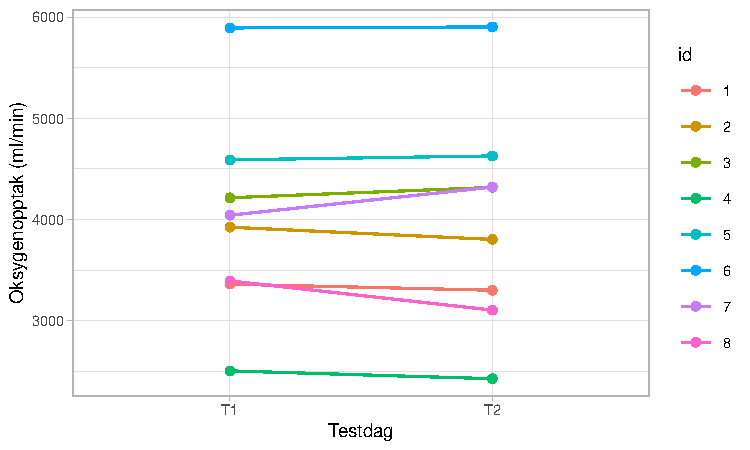
\includegraphics{Arbeidskrav-1_files/figure-pdf/fig-test-1.pdf}

}

\caption{\label{fig-test}Sammenligning av oksygenopptak målt i ml/min
mellom testdag 1 og testdag 2 for hver forsøksperson}

\end{figure}

\begin{figure}

{\centering 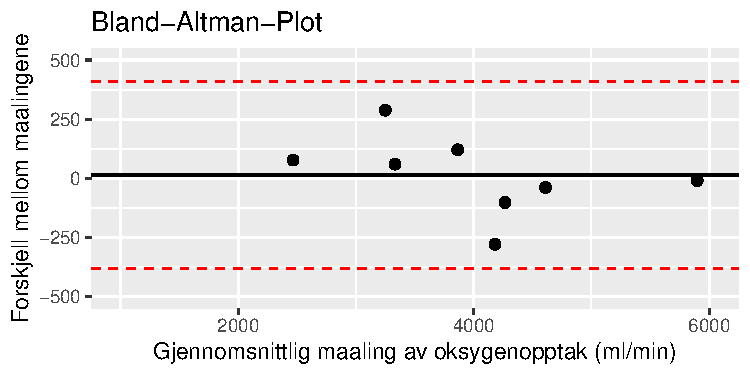
\includegraphics{Arbeidskrav-1_files/figure-pdf/fig-bland-1.pdf}

}

\caption{\label{fig-bland}Bland-Altman-Plot for maksimalt oksygenopptak
(ml/min). Stiplete linjer tilsvarer øvre og nedre limits of agreement.
Heltrukken linje tilsvarer gjennomsnittet av differansen mellom T1 og
T2}

\end{figure}

\newpage

\hypertarget{referanser}{%
\subsection*{Referanser}\label{referanser}}
\addcontentsline{toc}{subsection}{Referanser}

\hypertarget{refs}{}
\begin{CSLReferences}{1}{0}
\leavevmode\vadjust pre{\hypertarget{ref-halperinThreatsInternalValidity2015a}{}}%
Halperin, I., Pyne, D. B., \& Martin, D. T. (2015). Threats to
{Internal} {Validity} in {Exercise} {Science}: {A} {Review} of
{Overlooked} {Confounding} {Variables}. \emph{International Journal of
Sports Physiology and Performance}, \emph{10}(7), 823--829.
\url{https://doi.org/10.1123/ijspp.2014-0566}

\leavevmode\vadjust pre{\hypertarget{ref-hopkinsMeasuresReliabilitySports2000}{}}%
Hopkins, W. G. (2000). Measures of {Reliability} in {Sports} {Medicine}
and {Science}: \emph{Sports Medicine}, \emph{30}(1), 1--15.
\url{https://doi.org/10.2165/00007256-200030010-00001}

\leavevmode\vadjust pre{\hypertarget{ref-spiegelhalterArtStatisticsLearning2020}{}}%
Spiegelhalter, D. J. (2020b). \emph{The art of statistics: Learning from
data} (Paperback edition). Pelican Books.

\leavevmode\vadjust pre{\hypertarget{ref-spiegelhalter2020}{}}%
Spiegelhalter, D. J. (2020a). \emph{The art of statistics: learning from
data} (Published in paperback). Pelican, an imprint of Penguin Books.

\leavevmode\vadjust pre{\hypertarget{ref-tannerPhysiologicalTestsElite2013}{}}%
Tanner, R. K., Gore, C. J., \& Sport, A. I. of (Eds.). (2013).
\emph{Physiological tests for elite athletes} (2nd ed). Human Kinetics.

\end{CSLReferences}



\end{document}
